% vim: set textwidth=78 autoindent:

\pagenumbering{arabic}
\setcounter{page}{1}
\setcounter{secnumdepth}{1} 

%%%%% nothing to change above %%%%%%%%%%%%%%%

% when the revision of a section has been finalized, 
% comment out the following line:
%\updatedisclaimer

\section{Introducing GIS}\label{gis_intro}
\begin{tabular}{p{3.5cm}p{6cm}p{6cm}}
\multirow{2}{*}{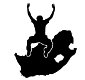
\includegraphics[width=2.5cm]{logo}} & Objectives: &
Understanding what GIS is and what it can be used for. \\ 
& & \\
& Keywords: & GIS, Computer, Maps, Data, Information System, Spatial,
Analysis \\
\hline
\end{tabular}

\subsection{Overview}

Just as we use a word processor to write documents and deal with words on a
computer, we can use a \textbf{GIS application} to deal with \textbf{spatial
information} on a computer. GIS stands for \textbf{'Geographical Information
System'}. A GIS consists of:

\begin{itemize}
\item \textbf{Digital Data} - the geographical information that you will view
and analyse using computer hardware and software.
\item \textbf{Computer Hardware} - computers used for storing data,
displaying graphics and processing data.
\item \textbf{Computer Software} - computer programs that run on the computer
hardware and allow you to work with digital data. A software program that
forms part of the GIS is called a GIS Application.
\end{itemize}

With a GIS application you can open digital maps on your computer, create new
spatial information to add to a map, create printed maps customised to your
needs and perform spatial analysis.

Let's look at a little example of how GIS can be useful. Imagine you are a
health worker and you make a note of the date and place of residence of every
patient you treat.

%% Note: xdvi does not show white text on black background but it works!
\begin{table}[ht]
\centering
\caption{Notes of date and place of residence of patients}\medskip
 \label{tab:diseases}
 \begin{tabular}{|p{3cm}|p{3cm}|p{3cm}|p{3cm}|}
 \hline 
 \rowcolor{black}
 \textcolor{white}{\textbf{Longitude}} &
 \textcolor{white}{\textbf{Latitude}} & 
 \textcolor{white}{\textbf{Disease}} &
 \textcolor{white}{\textbf{Date}} \\
 \hline 26.870436 & -31.909519 & Mumps & 13/12/2008 \\
 \hline 26.868682 & -31.909259 & Mumps & 24/12/2008 \\
 \hline 26.867707 & -31.910494 & Mumps & 22/01/2009 \\
 \hline 26.854908 & -31.920759 & Measles & 11/01/2009 \\
 \hline 26.855817 & -31.921929 & Measles & 26/01/2009 \\
 \hline 26.852764 & -31.921929 & Measles & 10/02/2009 \\
 \hline 26.852764 & -31.921929 & Measles & 22/02/2009 \\
 \hline 26.869072 & -31.911988 & Mumps & 02/02/2009 \\
 \hline 26.863354 & -31.916406 & Chicken Pox & 26/02/2009 \\
\hline
\end{tabular}
\end{table}

If you look at the table above you will quickly see that there were a lot of
measles cases in January and February. Our health worker recorded the
location of each patient's house by noting its latitude and longitude in the
table. Using this data in a GIS Application,  we can quickly understand a lot
more about the patterns of illness:

\begin{figure}[ht]
   \begin{center}
   \caption{Example showing disease records in a GIS application. It is easy
    to see that the mumps patients all live close to each other.}
\label{fig:disease_records}\smallskip
   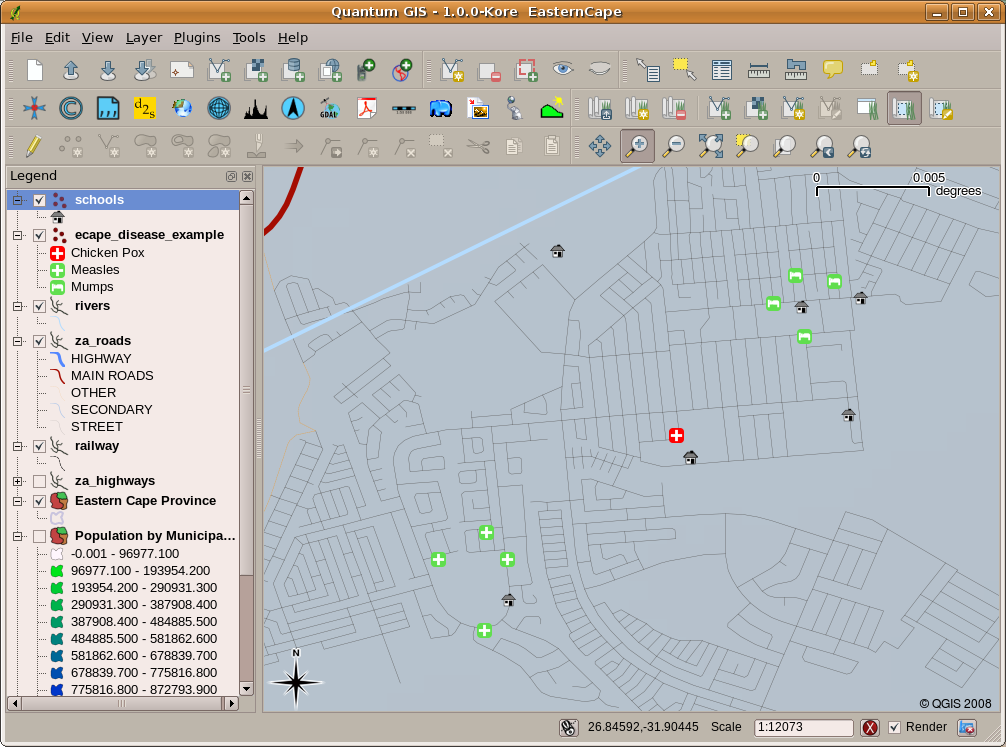
\includegraphics[clip=true, width=\textwidth]{ecape01}
\end{center}
\end{figure}

\subsection{More about GIS}\label{subsec:moreaboutGIS}

GIS is a relatively new field - it started in the 1970's. It used to be that
computerised GIS was only available to companies and universities that had
expensive computer equipment. These days, anyone with a personal computer or
laptop can use GIS software. Over time GIS Applications have also become
easier to use - it used to require a lot of training to use a GIS
Application, but now it is much easier to get started in GIS even for
amateurs and casual users. As we described above, GIS is more than just
software, it refers to all aspects of managing and using digital geographical
data. In the tutorials that follow we will be focusing on GIS Software.

\subsection{What is GIS Software / a GIS Application?}\label{subsec:whatisGIS}

You can see an example of what a \textbf{GIS Application} looks like in
Figure \ref{fig:disease_records} above. GIS Applications are normally
programs with a graphical user interface that can be manipulated using the
mouse and keyboard. The application provides \textbf{menus} near to the top
of the window (File, Edit etc.) which, when clicked using the mouse, show a
panel of \textbf{actions}. These actions provide a way for you to tell the
GIS Application what you want to do. For example you may use the menus to
tell the GIS Application to add a new layer to the display output.

\begin{figure}[ht]
   \begin{center}
   \caption{Application menus, when clicked with the mouse, expand to show a
   list of actions that can be carried out.}
   \label{fig:application_menu}\smallskip
   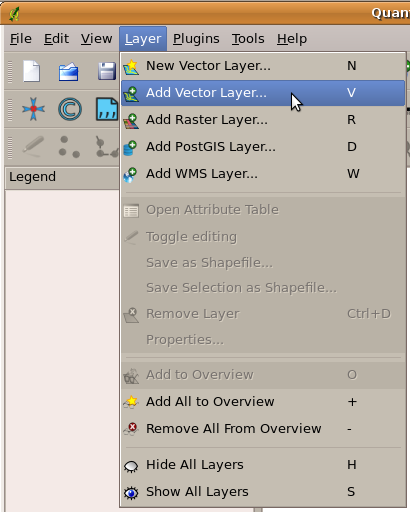
\includegraphics[clip=true, width=4cm]{topic1_menus}
\end{center}
\end{figure}

\textbf{Toolbars} (rows of small pictures that can be clicked with the mouse)
normally sit just below the menus and provide a quicker way to use frequently
needed actions.

\begin{figure}[ht]
   \begin{center}
   \caption{Toolbars provide quick access to commonly used functions. Holding
    your mouse over a picture will usually tell you what will happen when you
    click on it.}
   \label{fig:toolbars}\smallskip
   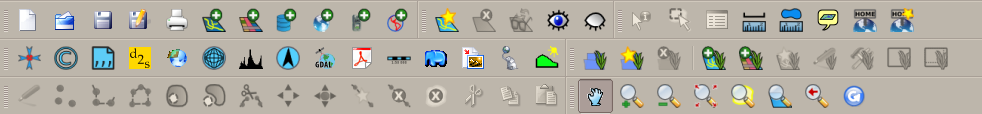
\includegraphics[clip=true, width=\textwidth]{topic1_toolbars}
\end{center}
\end{figure}

A common function of GIS Applications is to display \textbf{map layers}. Map
layers are stored as files on a disk or as records in a database. Normally
each map layer will represent something in the real world - a roads layer for
example will have data about the street network. 

When you open a layer in the GIS Application it will appear in the
\textbf{map view}. The map view shows a graphic representing your layer. When
you add more than one layer to a map view, the layers are overlaid on top of
each other. Figure \ref{fig:addlayer} below shows a map view that has several
layers being added to it. An important function of the map view is to allow
you to zoom in to magnify, zoom out to see a greater area and move around
(panning) in the map.

\begin{figure}[ht]
\centering
\caption{A map view with several layers being added to it}\label{fig:addlayer}
   \subfigure[A towns layer added to the map view]
   {\label{subfig:addlayer1}\fbox{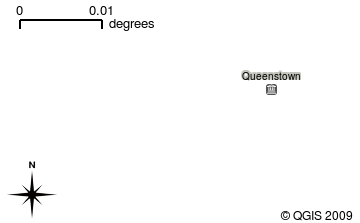
\includegraphics[clip=true, width=0.4\textwidth]{topic1_adding_layers1}}}\goodgap
   \subfigure[A schools layer added to the map view]
{\label{subfig:addlayer2}\fbox{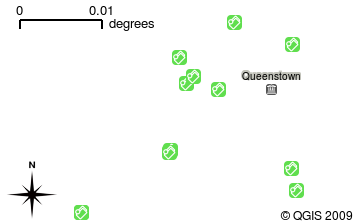
\includegraphics[clip=true, width=0.4\textwidth]{topic1_adding_layers2}}}\\
   \subfigure[A railways layer added to the map view]
{\label{subfig:addlayer3}\fbox{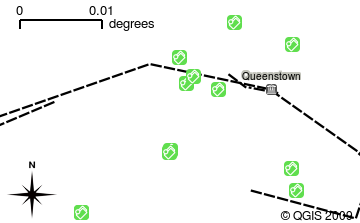
\includegraphics[clip=true, width=0.4\textwidth]{topic1_adding_layers3}}}\goodgap
   \subfigure[A rivers layer added to the map view] 
{\label{subfig:addlayer4}\fbox{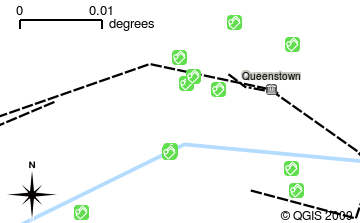
\includegraphics[clip=true, width=0.4\textwidth]{topic1_adding_layers4}}}
\end{figure}

Unlike paper maps, the maps displayed in GIS Applications can be changed
after they have been created. You can change the \textbf{symbology} of the
map layers to make them appear in different colours or symbols. 

\begin{figure}[ht]
\begin{center}
   \caption{GIS Software let you easily change symbology - the way
   information is displayed.}
   \label{fig:changesymbology}\smallskip
   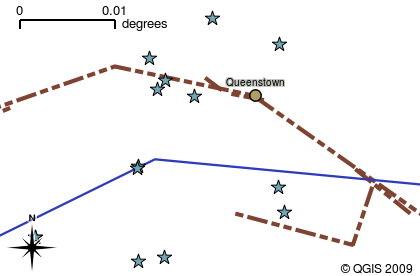
\includegraphics[clip=true, width=5.5cm]{topic1_changing_symbology}
\end{center}
\end{figure}

For example, if we take the map in Figure \ref{fig:addlayer}(d) and change
the symbology, we can completely change how it looks - as shown in Figure
\ref{fig:changesymbology}. Symbology plays an important role in how we
interpret maps, and GIS Applications are very good at letting you change
symbology quickly and easily.

Another common feature of GIS Applications is the \textbf{map legend}. The
map legend
provides a list of layers that have been loaded in the GIS Application.
Unlike a paper map legend, the map legend or 'layers list' in the GIS
Application provides a way to re-order, hide, show and group layers. Changing
the layer order is done by clicking on a layer in the legend, holding the
mouse button down and then dragging the layer to a new position. In
Figure \ref{fig:layerdrag}, the map legend is shown as the area to the left
of the GIS Application window. By changing the layer order, the way that
layers are drawn can be adjusted - in this case so that rivers are drawn over
the roads instead of below them.

\begin{figure}[h]
\centering
\caption{Changing the layer order allows to adjust the way that layers are
drawn}\label{fig:layerdrag}
   \subfigure[Before changing the layer order, rivers are drawn underneath
   roads]
   {\label{subfig:layerdrag1}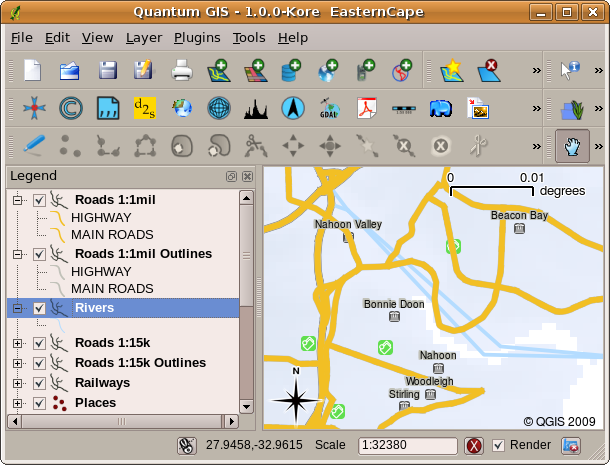
\includegraphics[clip=true, width=0.45\textwidth]{topic1_before_legend_drag}}\goodgap
   \subfigure[After changing the layer order, rivers are drawn on top of
   roads]
{\label{subfig:layerdrag2}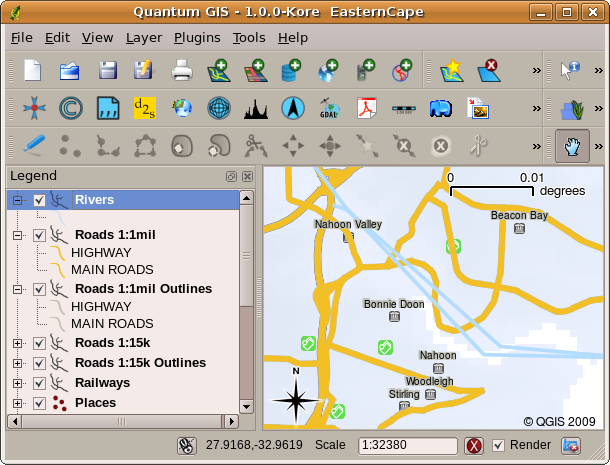
\includegraphics[clip=true, width=0.45\textwidth]{topic1_after_legend_drag}}
\end{figure}

\subsection{Getting a GIS Application for your own
computer(s)}\label{subsec:getagis}

There are many different GIS Applications available. Some have many
sophisticated features and cost tens of thousands of Rands for each copy. In
other cases, you can obtain a GIS Application for free. Deciding which GIS
Application to use is a question of how much money you can afford and
personal preference. For these tutorials, we will be using the Quantum GIS
Application, also known as QGIS. Quantum GIS is completely free and you can
copy it and share it with your friends as much as you like. If you received
this tutorial in printed form, you should have received a copy of QGIS with
it. If not, you can always visit \url{http://qgis.org} to download your free
copy if you have access to the internet.

\subsection{GIS Data}\label{subsec:gisdata}

Now that we know what a GIS is and what a GIS Application can do, let's talk
about \textbf{GIS data}. Data is another word for \textbf{information}. The
information we use in a GIS normally has a geographical aspect to it. Think
of our example above, about the health care worker. She created a table to
record diseases that looked like this:

%% Note: xdvi does not show white text on black background but it works!
\begin{table}[ht]
\centering
\caption{Example from table~\ref{tab:diseases} with date and place of
residence of patients}\medskip
 \begin{tabular}{|p{3cm}|p{3cm}|p{3cm}|p{3cm}|}
 \hline
 \rowcolor{black}
 \textcolor{white}{\textbf{Longitude}} &
 \textcolor{white}{\textbf{Latitude}} &
 \textcolor{white}{\textbf{Disease}} &
 \textcolor{white}{\textbf{Date}} \\
 \hline 26.870436 & -31.909519 & Mumps & 13/12/2008 \\
\hline
\end{tabular}
\end{table}

The longitude and latitude columns hold \textbf{geographical data}. The disease and
date columns hold \textbf{non-geographical data}. A common feature of GIS is that they
allow you to associate information (non-geographical data) with places
(geographical data). In fact, the GIS Application can store many pieces of
information which are associated with each place - something that paper maps
are not very good at. For example, our health care worker could store the
person's age and gender on her table. When the GIS Application draws the
layer, you can tell it to draw the layer based on gender, or based on disease
type, and so on. So, with a GIS Application we have a way to easily change
the appearance of the maps we created based on the non-geographical data
associated with places.

GIS Systems work with many different types of data. \textbf{Vector data} is stored as
a series of X,Y coordinate pairs inside the computer's memory. Vector data is
used to represent points, lines and areas. Figure \ref{fig:vectordata} shows
different types of vector data being viewed in a GIS application. In the
tutorials that follow we will be exploring vector data in more detail. 

\begin{figure}[ht]
   \begin{center}
   \caption{Vector data is used to represent points (e.g. towns), lines (e.g.
   rivers) and polygons (e.g. municipal boundaries).}
   \label{fig:vectordata}\smallskip
   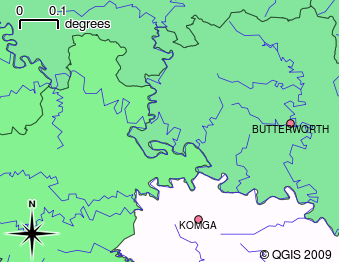
\includegraphics[clip=true, width=9cm]{topic1_vector_data}
\end{center}
\end{figure}

\textbf{Raster data} are stored as a grid of values. There are many satellites
circling the earth and the photographs they take are a kind of raster data
that can be viewed in a GIS. One important difference between raster and
vector data is that if you zoom in too much on a raster image, it will start
to appear 'blocky' (see Figure \ref{fig:rasterdata}). In fact these blocks
are the individual cells of the data grid that makes up the raster image. We
will be looking at raster data in greater detail in later tutorials.

\begin{figure}[h]
\centering
\caption{Zoom in to see the individual cells of the data grid that makes up
the raster image.}\label{fig:rasterdata}
   \subfigure[Raster data are often images taken by satellites. Here we can
   see mountains in the Eastern Cape.]
   {\label{subfig:layerdrag1}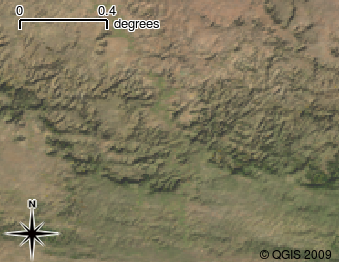
\includegraphics[clip=true, width=0.45\textwidth]{topic1_raster_data_zoomed_out}}\goodgap
   \subfigure[The same raster data, but this time zoomed in. The grid nature
   of the data can be seen]
{\label{subfig:layerdrag2}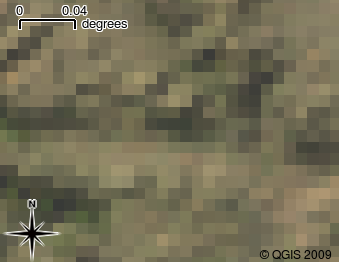
\includegraphics[clip=true, width=0.45\textwidth]{topic1_raster_data_zoomed_in}}
\end{figure}

\subsection{What have we learned?}

Let's wrap up what we covered in this worksheet:

\begin{itemize}
\item A \textbf{GIS} is a system of computer hardware, computer software and
geographical data.
\item A \textbf{GIS Application} allows you to view geographical data and is
an important part of the GIS.
\item A GIS Application normally consists of a \textbf{menu bar, toolbars}, a
\textbf{map view} and a \textbf{legend}. 
\item \textbf{Vector} and \textbf{raster} data are geographical data used in
a GIS application.
\item \textbf{Geographical} data can have associated \textbf{non-geographical} data.
\end{itemize}

\subsection{Now you try!}

Here are some ideas for you to try with your learners:

\begin{itemize}
\item \textbf{Geography}: Describe the concept of GIS to your learners as
outlined in this tutorial. Ask them to try to think of 3 reasons why it might
be handy to use a GIS instead of paper maps. Here are some that we could
think of:
\begin{itemize}
\item GIS Applications allow you to create many different types of maps from
the same data.
\item GIS is a great visualisation tool that can show you things about your
data and how they are related in space (e.g. those disease outbreaks we saw
earlier).
\item Paper maps need to be filed and are time consuming to view. The GIS can
hold a very large amount of map data and make it quick and easy to find a place
you are interested in.
\end{itemize}
\end{itemize}

\begin{itemize}
\item \textbf{Geography}: Can you and your learners think of how raster data
from satellites could be useful? Here are some ideas we had:
\begin{itemize}
\item During natural disasters, raster data can be useful to show where the
impacted areas are. For example a recent satellite image taken during a flood
can help to show where people may need rescuing.
\item Sometimes people do bad things to the the environment, like dumping
dangerous chemicals that kill plants and animals. Using raster data from
satellites can help us to monitor for these type of problems.
\item Town planners can use raster data from satellites to see where informal
settlements are and to help in planning infrastructure.
\end{itemize}
\end{itemize}

\subsection{Something to think about}

If you don't have a computer available, many of the topics we cover in this
tutorial can be reproduced using an overhead and transparency as it uses the
same technique of layering information. However, to properly understand GIS
it is always better to learn it using a computer.

\subsection{Further reading}

\textbf{Book}: Desktop GIS: Mapping the Planet with Open Source Tools.
\textbf{Author}: Gary Sherman. \textbf{ISBN}: 9781934356067 \cite{sherman08} 

\textbf{Website}: http://www.gisdevelopment.net/tutorials/tuman006.htm

The QGIS User Guide also has more detailed information on working with QGIS.

\subsection{What's next?}

In the sections that follow we are going to go into more detail, showing you
how to use a GIS Application. All of the tutorials will be done using QGIS.
Next up, let's look at vectors!

